Системы оптического распознавания позволяют включать в корпусы текста для обработки цифровые документы с неподготовленным текстовым слоем. 
Автором работы был разработан открытый программный пакет для языка python --- ShuemacherOCR, который позволяет выполнять
масштабный анализ русскоязычной естественно-научной методической литературы. Разработка специального пакета связана с особенностью составления печатных изданий.
Книги естественнонаучной тематики имеют существенно различающуюся верстку и содержат большое число иллюстраций, графиков и формул. Современные пакеты
для выполнения оптического распознания Nougat \cite{blecher2023nougat}, Tesseract \cite{smith2007overview} и LayoutParser  \cite{shen2021layoutparser} не вполне справляются
с распознанием таких документов, поскольку либо не поддерживают русский язык, либо не предназначены для работы с формулами.

В состав пакета входят модули как для обработки отдельных изображений, 
так и полноценных документов, позволяющие извлекать данные в структурированном виде. Для решения задачи пакет использует нейросетевые алгоритмы. 
Особенностью пакета  является возможность выделять в тексте на русском языке строчные математические формулы.
Установка выполняется из открытого реестра пакетов PyPI с помощью менеджера pip или из репозитория\footnote{\url{https://github.com/NMashalov/SchumacherOCR}}. 

Опишем процесс подготовки данных для обучения модуля оптического распознания. Начнем с принципиально описания процесса. 

\textit{Определение:} \textbf{Оптическое распознавание символов} (OCR) представляет собой процесс автоматического преобразования текста,
 представленного в виде изображения или сканированного документа, в текстовый формат.
 
В ходе оптического распознавания исходное изображение документа подвергается предварительной обработке. 
Корректируется ориентация изображения, подбирается оптимальная яркость, удаляются шумы. 
Следующим этапом является сегментация изображения, включающая разделение исходных изображений на отдельные символы или группы символов.
Далее при помощи алгоритмов распознавания, включающих методы машинного обучения и компьютерного зрения, 
символы на изображении анализируются и сопоставляются с соответствующими символами из набора знаков. 
На завершающем этапе распознавания символы объединяются в слова, предложения и абзацы, формируя полноценный текстовый документ. 
Точность и эффективность процедуры зависят от качества изображения, используемых алгоритмов распознавания, а также от языка и структуры текста.

Распознавание текста по изображению выполнялось на основе нейросети архитектуры Nougat \cite{blecher2023nougat}. Особенностью данной архитектуры является 
быстрая адаптация под новые виды данных и работа с изображением целиком, без необходимости промежуточного поиска регионов с текстом. 

Обучение сети проводилось на корпусе препринтов статей  \cite{clement2019use}, переведенных на русский язык с помощью интеллектуального 
ассистента ChatGPT \cite{ouyang2022training}.  Выбор был связан с возможностью сохранять оригинальную разметку TeX-документов. 

Для валидации результатов был разработан общедоступный корпус, позволяющий измерить качество распознавания 
\footnote{\url{https://huggingface.co/datasets/NMashalov/ru_educational_book_datasets}}. 

Разметка для обучения проводилось с помощью обращения к сервису компании MathPix. Метрики качества приведены в таблице 1 и сопоставимы с 
результатами, которые дает оригинальная модель Nougat.

\begin{table}
    \centering
    \begin{tabular}{||c | c | c||} 
     \hline
     \text{Параметр} & \text{Обучение} & \text{Валидация} \\
     \hline\hline
     \text{BLEU} & 83.2 & 80.4  \\ 
     \hline
     \text{Edit distance} & 0.15 & 0.17 \\
     \hline
    \end{tabular}
\end{table}


Автор продолжает развитие пакета и его адаптацию для среды распределенных вычислений,
использующих акторную модель взаимодействия между вычислителями.

\begin{figure}[h]
    \centering
    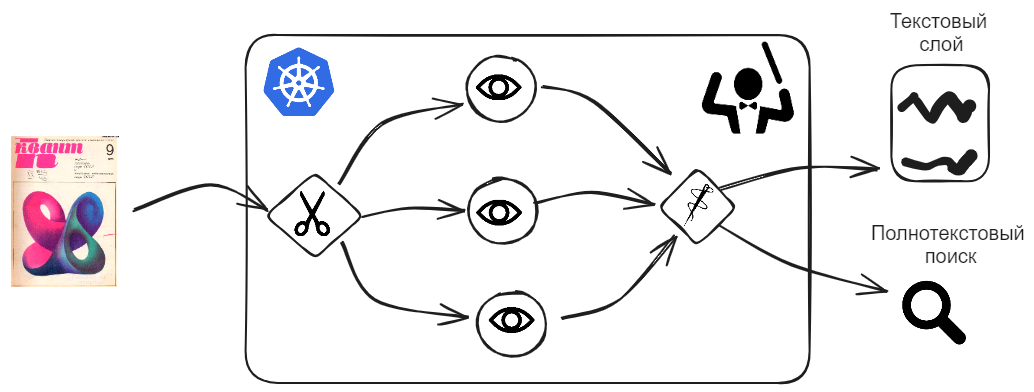
\includegraphics[width=0.7\textwidth]{assets/work/dataset/saga.excalidraw.png}
    \caption{Итоговая разметка выполняется посредством распределенных вычислений}
    \label{saga}
\end{figure}
